% Created by tikzDevice version 0.12.3.1 on 2021-05-24 11:49:00
% !TEX encoding = UTF-8 Unicode
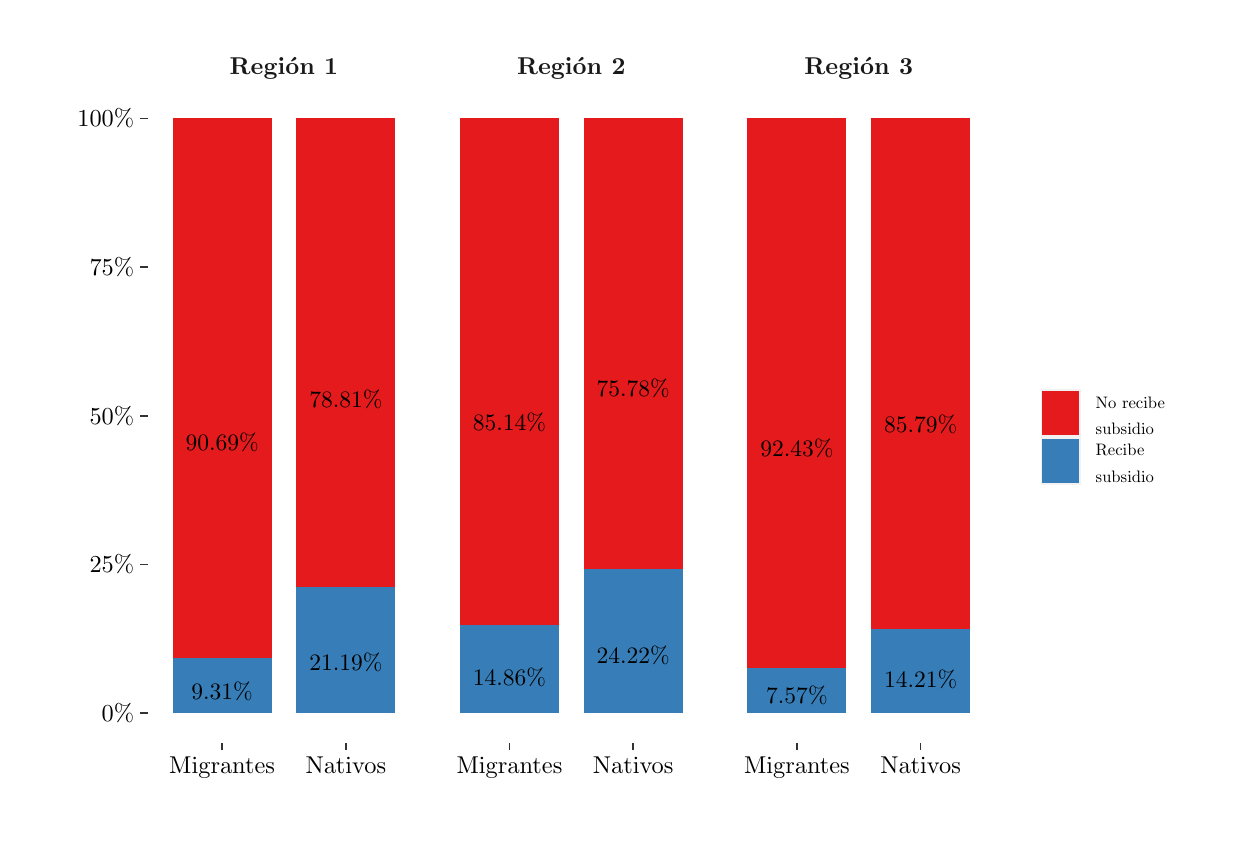
\begin{tikzpicture}[x=1pt,y=1pt]
\definecolor{fillColor}{RGB}{255,255,255}
\path[use as bounding box,fill=fillColor,fill opacity=0.00] (0,0) rectangle (433.62,289.08);
\begin{scope}
\path[clip] (  0.00,  0.00) rectangle (433.62,289.08);
\definecolor{drawColor}{RGB}{255,255,255}
\definecolor{fillColor}{RGB}{255,255,255}

\path[draw=drawColor,line width= 0.6pt,line join=round,line cap=round,fill=fillColor] (  0.00,  0.00) rectangle (433.62,289.08);
\end{scope}
\begin{scope}
\path[clip] ( 43.44, 30.69) rectangle (141.79,267.01);
\definecolor{drawColor}{RGB}{255,255,255}

\path[draw=drawColor,line width= 0.3pt,line join=round] ( 43.44, 68.28) --
	(141.79, 68.28);

\path[draw=drawColor,line width= 0.3pt,line join=round] ( 43.44,121.99) --
	(141.79,121.99);

\path[draw=drawColor,line width= 0.3pt,line join=round] ( 43.44,175.70) --
	(141.79,175.70);

\path[draw=drawColor,line width= 0.3pt,line join=round] ( 43.44,229.41) --
	(141.79,229.41);

\path[draw=drawColor,line width= 0.6pt,line join=round] ( 43.44, 41.43) --
	(141.79, 41.43);

\path[draw=drawColor,line width= 0.6pt,line join=round] ( 43.44, 95.14) --
	(141.79, 95.14);

\path[draw=drawColor,line width= 0.6pt,line join=round] ( 43.44,148.85) --
	(141.79,148.85);

\path[draw=drawColor,line width= 0.6pt,line join=round] ( 43.44,202.56) --
	(141.79,202.56);

\path[draw=drawColor,line width= 0.6pt,line join=round] ( 43.44,256.27) --
	(141.79,256.27);

\path[draw=drawColor,line width= 0.6pt,line join=round] ( 70.26, 30.69) --
	( 70.26,267.01);

\path[draw=drawColor,line width= 0.6pt,line join=round] (114.97, 30.69) --
	(114.97,267.01);
\definecolor{fillColor}{RGB}{228,26,28}

\path[fill=fillColor] ( 52.38, 61.44) rectangle ( 88.15,256.27);
\definecolor{fillColor}{RGB}{55,126,184}

\path[fill=fillColor] ( 52.38, 41.43) rectangle ( 88.15, 61.44);
\definecolor{fillColor}{RGB}{228,26,28}

\path[fill=fillColor] ( 97.09, 86.94) rectangle (132.85,256.27);
\definecolor{fillColor}{RGB}{55,126,184}

\path[fill=fillColor] ( 97.09, 41.43) rectangle (132.85, 86.94);
\definecolor{drawColor}{RGB}{0,0,0}

\node[text=drawColor,anchor=base,inner sep=0pt, outer sep=0pt, scale=  0.85] at ( 70.26,136.43) {90.69{\%}};

\node[text=drawColor,anchor=base,inner sep=0pt, outer sep=0pt, scale=  0.85] at ( 70.26, 46.49) {9.31{\%}};

\node[text=drawColor,anchor=base,inner sep=0pt, outer sep=0pt, scale=  0.85] at (114.97,151.73) {78.81{\%}};

\node[text=drawColor,anchor=base,inner sep=0pt, outer sep=0pt, scale=  0.85] at (114.97, 56.70) {21.19{\%}};
\end{scope}
\begin{scope}
\path[clip] (147.29, 30.69) rectangle (245.64,267.01);
\definecolor{drawColor}{RGB}{255,255,255}

\path[draw=drawColor,line width= 0.3pt,line join=round] (147.29, 68.28) --
	(245.64, 68.28);

\path[draw=drawColor,line width= 0.3pt,line join=round] (147.29,121.99) --
	(245.64,121.99);

\path[draw=drawColor,line width= 0.3pt,line join=round] (147.29,175.70) --
	(245.64,175.70);

\path[draw=drawColor,line width= 0.3pt,line join=round] (147.29,229.41) --
	(245.64,229.41);

\path[draw=drawColor,line width= 0.6pt,line join=round] (147.29, 41.43) --
	(245.64, 41.43);

\path[draw=drawColor,line width= 0.6pt,line join=round] (147.29, 95.14) --
	(245.64, 95.14);

\path[draw=drawColor,line width= 0.6pt,line join=round] (147.29,148.85) --
	(245.64,148.85);

\path[draw=drawColor,line width= 0.6pt,line join=round] (147.29,202.56) --
	(245.64,202.56);

\path[draw=drawColor,line width= 0.6pt,line join=round] (147.29,256.27) --
	(245.64,256.27);

\path[draw=drawColor,line width= 0.6pt,line join=round] (174.11, 30.69) --
	(174.11,267.01);

\path[draw=drawColor,line width= 0.6pt,line join=round] (218.81, 30.69) --
	(218.81,267.01);
\definecolor{fillColor}{RGB}{228,26,28}

\path[fill=fillColor] (156.23, 73.34) rectangle (191.99,256.27);
\definecolor{fillColor}{RGB}{55,126,184}

\path[fill=fillColor] (156.23, 41.43) rectangle (191.99, 73.34);
\definecolor{fillColor}{RGB}{228,26,28}

\path[fill=fillColor] (200.93, 93.47) rectangle (236.70,256.27);
\definecolor{fillColor}{RGB}{55,126,184}

\path[fill=fillColor] (200.93, 41.43) rectangle (236.70, 93.47);
\definecolor{drawColor}{RGB}{0,0,0}

\node[text=drawColor,anchor=base,inner sep=0pt, outer sep=0pt, scale=  0.85] at (174.11,143.57) {85.14{\%}};

\node[text=drawColor,anchor=base,inner sep=0pt, outer sep=0pt, scale=  0.85] at (174.11, 51.25) {14.86{\%}};

\node[text=drawColor,anchor=base,inner sep=0pt, outer sep=0pt, scale=  0.85] at (218.81,155.65) {75.78{\%}};

\node[text=drawColor,anchor=base,inner sep=0pt, outer sep=0pt, scale=  0.85] at (218.81, 59.30) {24.22{\%}};
\end{scope}
\begin{scope}
\path[clip] (251.14, 30.69) rectangle (349.48,267.01);
\definecolor{drawColor}{RGB}{255,255,255}

\path[draw=drawColor,line width= 0.3pt,line join=round] (251.14, 68.28) --
	(349.48, 68.28);

\path[draw=drawColor,line width= 0.3pt,line join=round] (251.14,121.99) --
	(349.48,121.99);

\path[draw=drawColor,line width= 0.3pt,line join=round] (251.14,175.70) --
	(349.48,175.70);

\path[draw=drawColor,line width= 0.3pt,line join=round] (251.14,229.41) --
	(349.48,229.41);

\path[draw=drawColor,line width= 0.6pt,line join=round] (251.14, 41.43) --
	(349.48, 41.43);

\path[draw=drawColor,line width= 0.6pt,line join=round] (251.14, 95.14) --
	(349.48, 95.14);

\path[draw=drawColor,line width= 0.6pt,line join=round] (251.14,148.85) --
	(349.48,148.85);

\path[draw=drawColor,line width= 0.6pt,line join=round] (251.14,202.56) --
	(349.48,202.56);

\path[draw=drawColor,line width= 0.6pt,line join=round] (251.14,256.27) --
	(349.48,256.27);

\path[draw=drawColor,line width= 0.6pt,line join=round] (277.96, 30.69) --
	(277.96,267.01);

\path[draw=drawColor,line width= 0.6pt,line join=round] (322.66, 30.69) --
	(322.66,267.01);
\definecolor{fillColor}{RGB}{228,26,28}

\path[fill=fillColor] (260.08, 57.70) rectangle (295.84,256.27);
\definecolor{fillColor}{RGB}{55,126,184}

\path[fill=fillColor] (260.08, 41.43) rectangle (295.84, 57.70);
\definecolor{fillColor}{RGB}{228,26,28}

\path[fill=fillColor] (304.78, 71.95) rectangle (340.54,256.27);
\definecolor{fillColor}{RGB}{55,126,184}

\path[fill=fillColor] (304.78, 41.43) rectangle (340.54, 71.95);
\definecolor{drawColor}{RGB}{0,0,0}

\node[text=drawColor,anchor=base,inner sep=0pt, outer sep=0pt, scale=  0.85] at (277.96,134.19) {92.43{\%}};

\node[text=drawColor,anchor=base,inner sep=0pt, outer sep=0pt, scale=  0.85] at (277.96, 45.00) {7.57{\%}};

\node[text=drawColor,anchor=base,inner sep=0pt, outer sep=0pt, scale=  0.85] at (322.66,142.74) {85.79{\%}};

\node[text=drawColor,anchor=base,inner sep=0pt, outer sep=0pt, scale=  0.85] at (322.66, 50.70) {14.21{\%}};
\end{scope}
\begin{scope}
\path[clip] ( 43.44,267.01) rectangle (141.79,283.58);
\definecolor{drawColor}{gray}{0.10}

\node[text=drawColor,anchor=base,inner sep=0pt, outer sep=0pt, scale=  0.88] at ( 92.62,272.26) {\textbf{Región 1}};
\end{scope}
\begin{scope}
\path[clip] (147.29,267.01) rectangle (245.64,283.58);
\definecolor{drawColor}{gray}{0.10}

\node[text=drawColor,anchor=base,inner sep=0pt, outer sep=0pt, scale=  0.88] at (196.46,272.26) {\textbf{Región 2}};
\end{scope}
\begin{scope}
\path[clip] (251.14,267.01) rectangle (349.48,283.58);
\definecolor{drawColor}{gray}{0.10}

\node[text=drawColor,anchor=base,inner sep=0pt, outer sep=0pt, scale=  0.88] at (300.31,272.26) {\textbf{Región 3}};
\end{scope}
\begin{scope}
\path[clip] (  0.00,  0.00) rectangle (433.62,289.08);
\definecolor{drawColor}{gray}{0.20}

\path[draw=drawColor,line width= 0.6pt,line join=round] ( 70.26, 27.94) --
	( 70.26, 30.69);

\path[draw=drawColor,line width= 0.6pt,line join=round] (114.97, 27.94) --
	(114.97, 30.69);
\end{scope}
\begin{scope}
\path[clip] (  0.00,  0.00) rectangle (433.62,289.08);
\definecolor{drawColor}{RGB}{0,0,0}

\node[text=drawColor,anchor=base,inner sep=0pt, outer sep=0pt, scale=  0.88] at ( 70.26, 19.68) {Migrantes};

\node[text=drawColor,anchor=base,inner sep=0pt, outer sep=0pt, scale=  0.88] at (114.97, 19.68) {Nativos};
\end{scope}
\begin{scope}
\path[clip] (  0.00,  0.00) rectangle (433.62,289.08);
\definecolor{drawColor}{gray}{0.20}

\path[draw=drawColor,line width= 0.6pt,line join=round] (174.11, 27.94) --
	(174.11, 30.69);

\path[draw=drawColor,line width= 0.6pt,line join=round] (218.81, 27.94) --
	(218.81, 30.69);
\end{scope}
\begin{scope}
\path[clip] (  0.00,  0.00) rectangle (433.62,289.08);
\definecolor{drawColor}{RGB}{0,0,0}

\node[text=drawColor,anchor=base,inner sep=0pt, outer sep=0pt, scale=  0.88] at (174.11, 19.68) {Migrantes};

\node[text=drawColor,anchor=base,inner sep=0pt, outer sep=0pt, scale=  0.88] at (218.81, 19.68) {Nativos};
\end{scope}
\begin{scope}
\path[clip] (  0.00,  0.00) rectangle (433.62,289.08);
\definecolor{drawColor}{gray}{0.20}

\path[draw=drawColor,line width= 0.6pt,line join=round] (277.96, 27.94) --
	(277.96, 30.69);

\path[draw=drawColor,line width= 0.6pt,line join=round] (322.66, 27.94) --
	(322.66, 30.69);
\end{scope}
\begin{scope}
\path[clip] (  0.00,  0.00) rectangle (433.62,289.08);
\definecolor{drawColor}{RGB}{0,0,0}

\node[text=drawColor,anchor=base,inner sep=0pt, outer sep=0pt, scale=  0.88] at (277.96, 19.68) {Migrantes};

\node[text=drawColor,anchor=base,inner sep=0pt, outer sep=0pt, scale=  0.88] at (322.66, 19.68) {Nativos};
\end{scope}
\begin{scope}
\path[clip] (  0.00,  0.00) rectangle (433.62,289.08);
\definecolor{drawColor}{RGB}{0,0,0}

\node[text=drawColor,anchor=base east,inner sep=0pt, outer sep=0pt, scale=  0.88] at ( 38.49, 38.40) {0{\%}};

\node[text=drawColor,anchor=base east,inner sep=0pt, outer sep=0pt, scale=  0.88] at ( 38.49, 92.11) {25{\%}};

\node[text=drawColor,anchor=base east,inner sep=0pt, outer sep=0pt, scale=  0.88] at ( 38.49,145.82) {50{\%}};

\node[text=drawColor,anchor=base east,inner sep=0pt, outer sep=0pt, scale=  0.88] at ( 38.49,199.53) {75{\%}};

\node[text=drawColor,anchor=base east,inner sep=0pt, outer sep=0pt, scale=  0.88] at ( 38.49,253.24) {100{\%}};
\end{scope}
\begin{scope}
\path[clip] (  0.00,  0.00) rectangle (433.62,289.08);
\definecolor{drawColor}{gray}{0.20}

\path[draw=drawColor,line width= 0.6pt,line join=round] ( 40.69, 41.43) --
	( 43.44, 41.43);

\path[draw=drawColor,line width= 0.6pt,line join=round] ( 40.69, 95.14) --
	( 43.44, 95.14);

\path[draw=drawColor,line width= 0.6pt,line join=round] ( 40.69,148.85) --
	( 43.44,148.85);

\path[draw=drawColor,line width= 0.6pt,line join=round] ( 40.69,202.56) --
	( 43.44,202.56);

\path[draw=drawColor,line width= 0.6pt,line join=round] ( 40.69,256.27) --
	( 43.44,256.27);
\end{scope}
\begin{scope}
\path[clip] (  0.00,  0.00) rectangle (433.62,289.08);
\definecolor{fillColor}{RGB}{255,255,255}

\path[fill=fillColor] (360.48,118.46) rectangle (428.12,179.23);
\end{scope}
\begin{scope}
\path[clip] (  0.00,  0.00) rectangle (433.62,289.08);
\definecolor{fillColor}{gray}{0.95}

\path[fill=fillColor] (365.98,141.24) rectangle (380.44,158.52);
\end{scope}
\begin{scope}
\path[clip] (  0.00,  0.00) rectangle (433.62,289.08);
\definecolor{fillColor}{RGB}{228,26,28}

\path[fill=fillColor] (366.69,141.95) rectangle (379.73,157.80);
\end{scope}
\begin{scope}
\path[clip] (  0.00,  0.00) rectangle (433.62,289.08);
\definecolor{fillColor}{gray}{0.95}

\path[fill=fillColor] (365.98,123.96) rectangle (380.44,141.24);
\end{scope}
\begin{scope}
\path[clip] (  0.00,  0.00) rectangle (433.62,289.08);
\definecolor{fillColor}{RGB}{55,126,184}

\path[fill=fillColor] (366.69,124.68) rectangle (379.73,140.53);
\end{scope}
\begin{scope}
\path[clip] (  0.00,  0.00) rectangle (433.62,289.08);
\definecolor{drawColor}{RGB}{0,0,0}

\node[text=drawColor,anchor=base west,inner sep=0pt, outer sep=0pt, scale=  0.60] at (385.94,151.60) {No recibe};

\node[text=drawColor,anchor=base west,inner sep=0pt, outer sep=0pt, scale=  0.60] at (385.94,142.10) {subsidio};
\end{scope}
\begin{scope}
\path[clip] (  0.00,  0.00) rectangle (433.62,289.08);
\definecolor{drawColor}{RGB}{0,0,0}

\node[text=drawColor,anchor=base west,inner sep=0pt, outer sep=0pt, scale=  0.60] at (385.94,134.32) {Recibe};

\node[text=drawColor,anchor=base west,inner sep=0pt, outer sep=0pt, scale=  0.60] at (385.94,124.82) {subsidio};
\end{scope}
\end{tikzpicture}
